\newpage
\section{Solid discretization: combining SPH and DEM}
\label{sec:solid-discretization}

The purpose of this Section is to devise a framework where the dynamics of solid bodies of arbitrary shape can be discretized in a way that solid-fluid interactions become trivial in the context of the fluid discretization presented in Section \ref{sec:fluid-discretization}. Section \ref{sec:solid-discretization_body} presents that general framework, where discrete equations for rigid body dynamics are introduced, generalizing the source of accelerations affecting a body. 

The \ac{DEM} model is introduced in Section \ref{sec:solid-discretization_force}, where the particular case of solid-solid interaction is explored. Traditional \ac{DEM} models are analyzed, as well as their numerical properties.

The result of this section is a \ac{DCDEM}, fully respecting the requirements of an accurate and robust model for the treatment of solid bodies with 6 \ac{DOF} in a multiphase setting.


\subsection{Rigid body discretization}
\label{sec:solid-discretization_body}

In the domain frame reference, the equations for a rigid body $I$ can be written as
%
\begin{equation} \label{eq:rigid_linear_newton}
	M_I\frac{d\ve{V}_I}{dt}=\sum_i \ve{F_i}
\end{equation}

\begin{equation} \label{eq:rigid_angular_newton}
	\ve{I}_I\frac{d\ve{\Omega}_I}{dt}=\sum_i(\ve{r}_i-\ve{R}_I)\times \ve{F_i},
\end{equation}
%
where body $I$ possesses a mass $M_I$, velocity $\boldsymbol{V}_I$, inertial tensor $\boldsymbol{I}_I$, angular velocity $\boldsymbol{\Omega}_I$ and center of gravity $\boldsymbol{R}_I$, and is subjected to an arbitrary number of forces $\ve{F_i}$, applied at points $\ve{r_i}$. 

In a particulate method it is trivial to idealize sub sets of particles in the domain whose variables are integrated in time with a different set of equations. If one uses Newton's equations for rigid body dynamics, then, that system of particles represents a rigid body. If body $I$ is a collection of particles\footnote{In this section $I$ is used for both the index of the rigid body in question and as the set of indexes from the particles that constitute the body. The abuse of notation is employed since in this context, they are semantically coincident.}, then the right side of Equations \eqref{eq:rigid_linear_newton} and \eqref{eq:rigid_angular_newton} can easily be discretized by

%
\begin{equation} \label{eq:rigid_linear}
	M_I\frac{d\ve{V}_I}{dt}=\sum_{k\in I} m_k \frac{{d{\ve{u}_k}}}{{dt}}
\end{equation}
%
\begin{equation} \label{eq:rigid_angular}
	\ve{I}_I\frac{d\ve{\Omega}_I}{dt}=\sum_{k\in I}m_k(\ve{r}_k-\ve{R}_I)\times \frac{{d{\ve{v}_k}}}{{dt}}
\end{equation}
%
$m_k {{d{\boldsymbol{u}_k}}}/{{dt}}$ represents the force by unit mass applied to particle $k$, belonging to body $I$. This force encompasses body forces (gravity), fluid resultants as well as the result of any rigid contact that might occur. This is inline with the work of \cite{Koshizuka-1998}, that first applied this idea in the context of \ac{MPS}.

Expressions \eqref{eq:rigid_linear} and \eqref{eq:rigid_angular} are obtained directly from applying \eqref{eq:rigid_linear_newton} and \eqref{eq:rigid_angular_newton} to a system of particles, i.e., they inherently conserve linear and angular momentum, as they are simple conservation laws. This is an advantage of particulate Lagrangian discretizations, since they are an exact representation of particle systems if the closure terms are also exact. For this system, it is simple to write the center of mass $\ve{R}_I$ and inertia tensor $\ve{I}_I$

%
\begin{equation} \label{eq:rigid_center_inertia}
	\ve{R}_I=\frac{1}{n_I}\sum_{k\in I} \ve{R}_k; \;\;\;\;\;\;\; \ve{I}_I=\sum_{k\in I}=m_k[\ve{r}_k-\ve{R}_I][\ve{r}_k-\ve{R}_I]
\end{equation}
%
where $n_I$ is them number of particles that constitute body $I$, $[\ve{r}_k-\ve{R}_I]$ is the skew-symmetric matrix built from $\ve{r}_k-\ve{R}_I$. Keeping in the domain frame reference implies that these quantities need to be recomputed whenever the system suffers an acceleration. 

Forces resulting from solid-fluid interaction are computed with Equation \eqref{eq:sph_navier_momentum_I}, where the viscous formulation provides a viscous drag closure. No \textit{ad-hoc} terms are added, since all the dynamics are a result of the fundamental, particle-wise, solution of Equations \eqref{eq:rigid_linear} and \eqref{eq:rigid_angular}.

This formulation can be seen as an extension of the dynamic boundary conditions introduced in Section \ref{sec:BCs}. As such, it suffers from the same overestimation of the density across the fluid/solid interface \cite{Price-2008,Saitoh-2013}, resulting from an entropy jump. The inclusion of the $\delta$-SPH diffusive term in Equation \eqref{eq:sph_navier_cont_delta_sph} allows for an apparently correct density estimation across the interface, as explored in the Results Section. The particles belonging to body $I$ are then moved according to

%
\begin{equation} \label{eq:rigid_propag_vel}
	\ve{u}_k= \ve{V}_I+\ve{\Omega}_I \times (\ve{r}_k-\ve{R}_I),
\end{equation}
%
\textit{i.e.}, the velocity given by propagating the rigid body velocities.


\subsection{Force discretization: the DEM model}
\label{sec:solid-discretization_force}

Forces $m_k {{d{\boldsymbol{u}_k}}}/{{dt}}$ will rise whenever a particle interacts with another. In the particular case of a solid-solid collision, the contact force is decomposed into $\ve{F}_n$ and $\ve{F}_t$, normal and tangential components respectively. Both of these forces will take forms explored in Section \ref{sec:solid_model}, with the addition of viscous dissipation effects. This is because two colliding bodies undergo a deformation which will be somewhere between perfectly inelastic and perfectly elastic, usually quantified by the normal restitution coefficient

%
\begin{equation} \label{eq:rest_coeff_def}
	e_n=-\frac{v_n|_{t=t^n}}{v_n|_{t=0}}, \;\;\;\; e\in[0,1]
\end{equation}
%
where $t=t^n$ is the instant at the end of collision and $t=0$ is the instant immediately before.

Forces are further decomposed into a repulsion force, $\boldsymbol{F}^r$, arising from the elastic deformation of the material, and a damping force, $\boldsymbol{F}^d$, for the viscous dissipation of energy during the deformation. Other dissipative mechanisms, such as plastic deformation and emission of elastic waves, excited from impact, will not be considered. The elastic waves are always present, but carry very little energy \citep{Shaefer-1996}, and are usually disregarded. Plastic deformation is not considered directly as its effects can, to some extent, be included in the viscous dissipation terms.

Figure \ref{fig:dem_scheme} generally illustrates the proposed viscoelastic DEM mechanism between two interacting particles.

%
\begin{figure}[ht!]
	\centering
	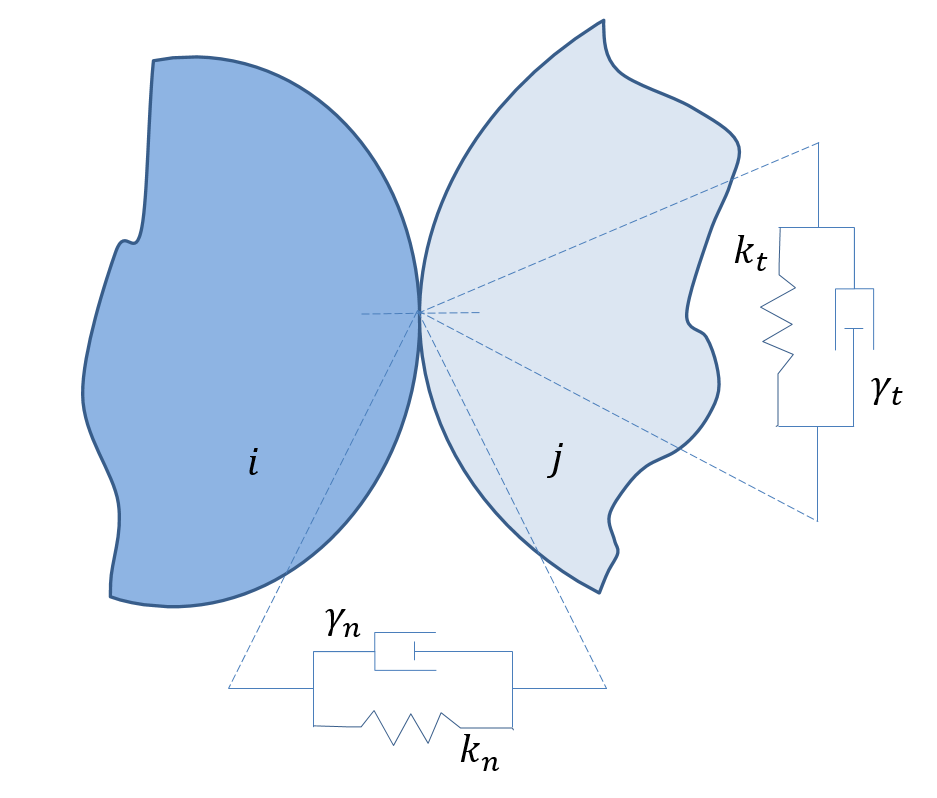
\includegraphics[width=0.60\linewidth]{Figures/3.Chapter/DEM_contacts}
	\caption{Scheme of DEM mechanism.}
	\label{fig:dem_scheme} 
\end{figure}
%
Every interaction is conceptualized as a system of springs and dampers. A general expression for the normal force in such viscoelastic model will be

%
\begin{equation} \label{eq:normal_viscoelastic_I}
	\ve{F}_{n,ij}=\ve{F}_n^r+\ve{F}_n^d=k_{n,ij}\delta_{ij}^{p_1}\ve{e}_{ij}-\gamma_{n,ij}\delta_{ij}^{p_2}\dot{\delta}_{ij}\ve{e}_{ij},
\end{equation}
%
where $k_{n,ij}$ is the normal stiffness constant of pair $ij$, $\delta_{ij}=\max(0, (d_i+d_j)/2-|\ve{r_{ij}}|)$ is the particle overlap, $\ve{e}_{ij}$ is the unit vector between the two mass centers and $\gamma_{n,ij}$ is the normal damping constant. For $p_1=p_2=1$, the mechanism is linear, corresponding to a simple damped harmonic resonator. An analytical solution \citep{Shaefer-1996} shows that this leads to a constant normal restitution coefficient, independent of the impact velocity

%
\begin{equation} \label{eq:linear_restitution_coeff}
	e_{n,ij}=\exp\left( -\frac{\gamma_{n,ij}}{2M^*}t_{c,ij} \right)
\end{equation}
%
where $M^*={m_im_j}/({m_i+m_j})$ and $t_{c,ij}$ is the contact duration, given by

%
\begin{equation} \label{eq:linear_tc}
	t_{c,ij}=\pi \left( \frac{k_{n,ij}}{M^*}- \left( \frac{\gamma_{n,ij}}{2M^*} \right)^2 \right)^{-1/2}
\end{equation}
%
Experimental studies using pendulum devices indicate that the $e_n$ and $t_c$ should depend on impact velocity however. Figures \ref{fig:Restitution_coeff} and \ref{fig:t_c_exp} both compiled by \cite{Kruggel-Emden-2007}, show that dramatic variations of these quantities may be registered.

%
\begin{figure}[ht!]
	\centering
	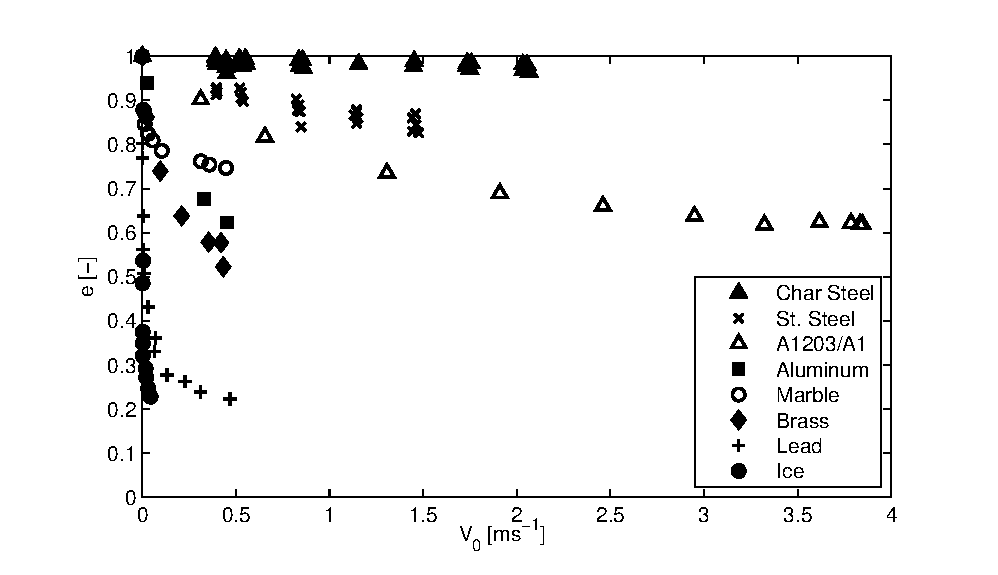
\includegraphics[width=0.73\linewidth]{Figures/3.Chapter/e_vo}
	\caption{Restitution coefficient $e$ as a function of initial normal velocity $V_0$ \citep{Kruggel-Emden-2007}.}
	\label{fig:Restitution_coeff} 
\end{figure}
%

%
%\begin{figure}[ht!]
%	\centering
%	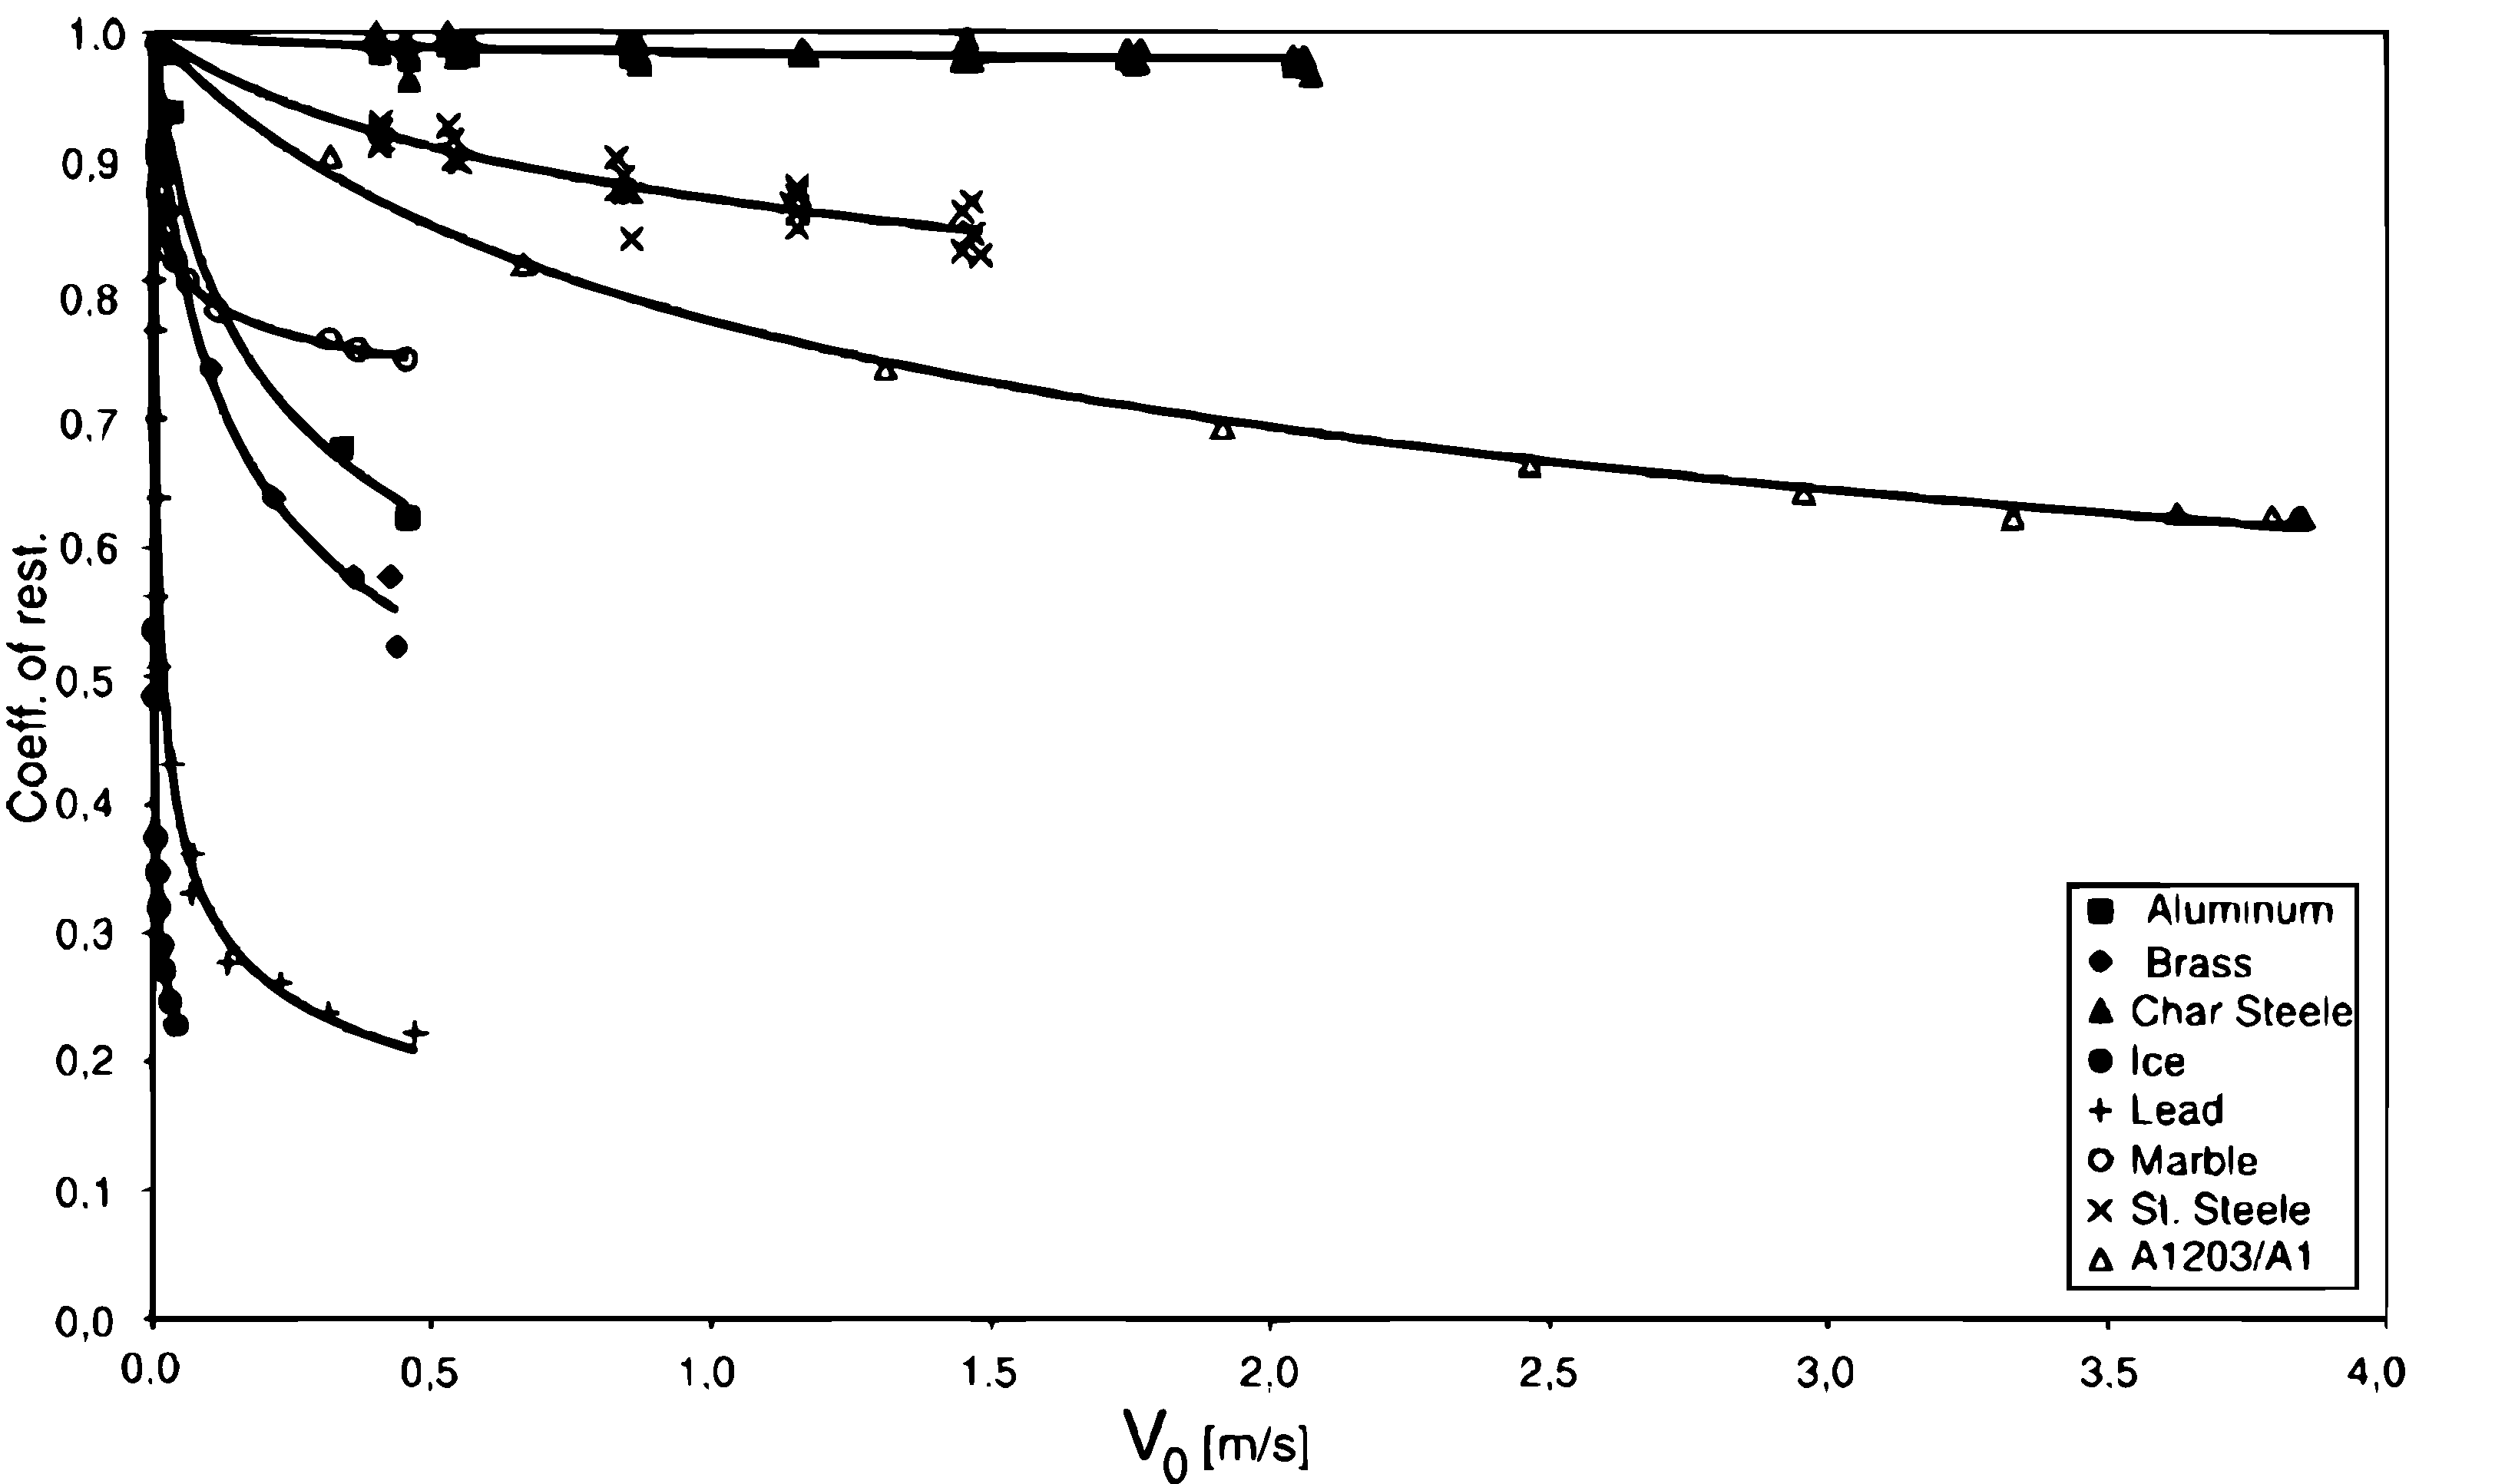
\includegraphics[width=0.80\linewidth]{Figures/3.Chapter/rest_coeff_exp}
%	\caption{Restitution coefficient $e$ as a function of impact normal velocity $V_0$ \citep{Kruggel-Emden-2007}.}
%	\label{fig:Restitution_coeff} 
%\end{figure}
%
%
\begin{figure}[ht!]
	\centering
	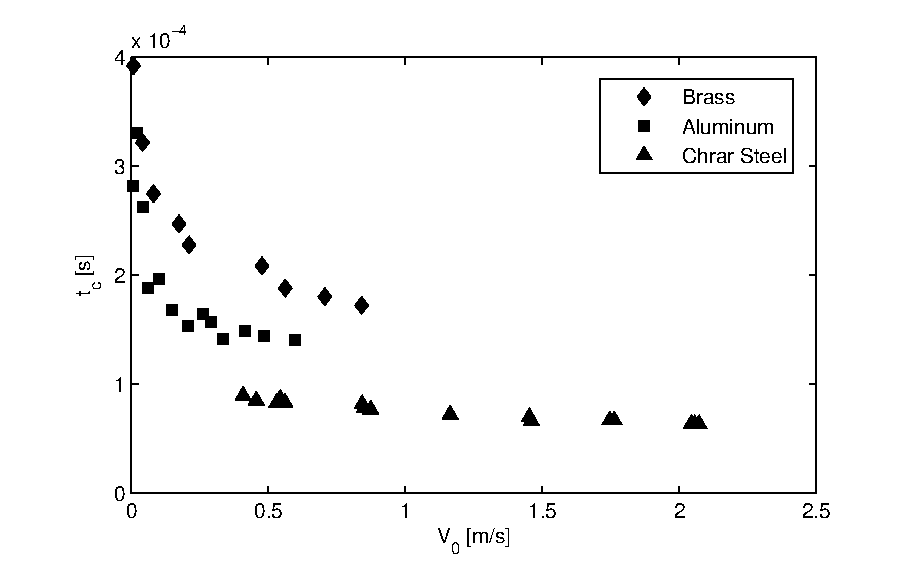
\includegraphics[width=0.70\linewidth]{Figures/3.Chapter/tc_vo}
	\caption{Duration of contact $t_c$ as a function of the impact normal velocity $V_0$ \citep{Kruggel-Emden-2007}.}
	\label{fig:t_c_exp} 
\end{figure}
%
%
%\begin{figure}[ht!]
%	\centering
%	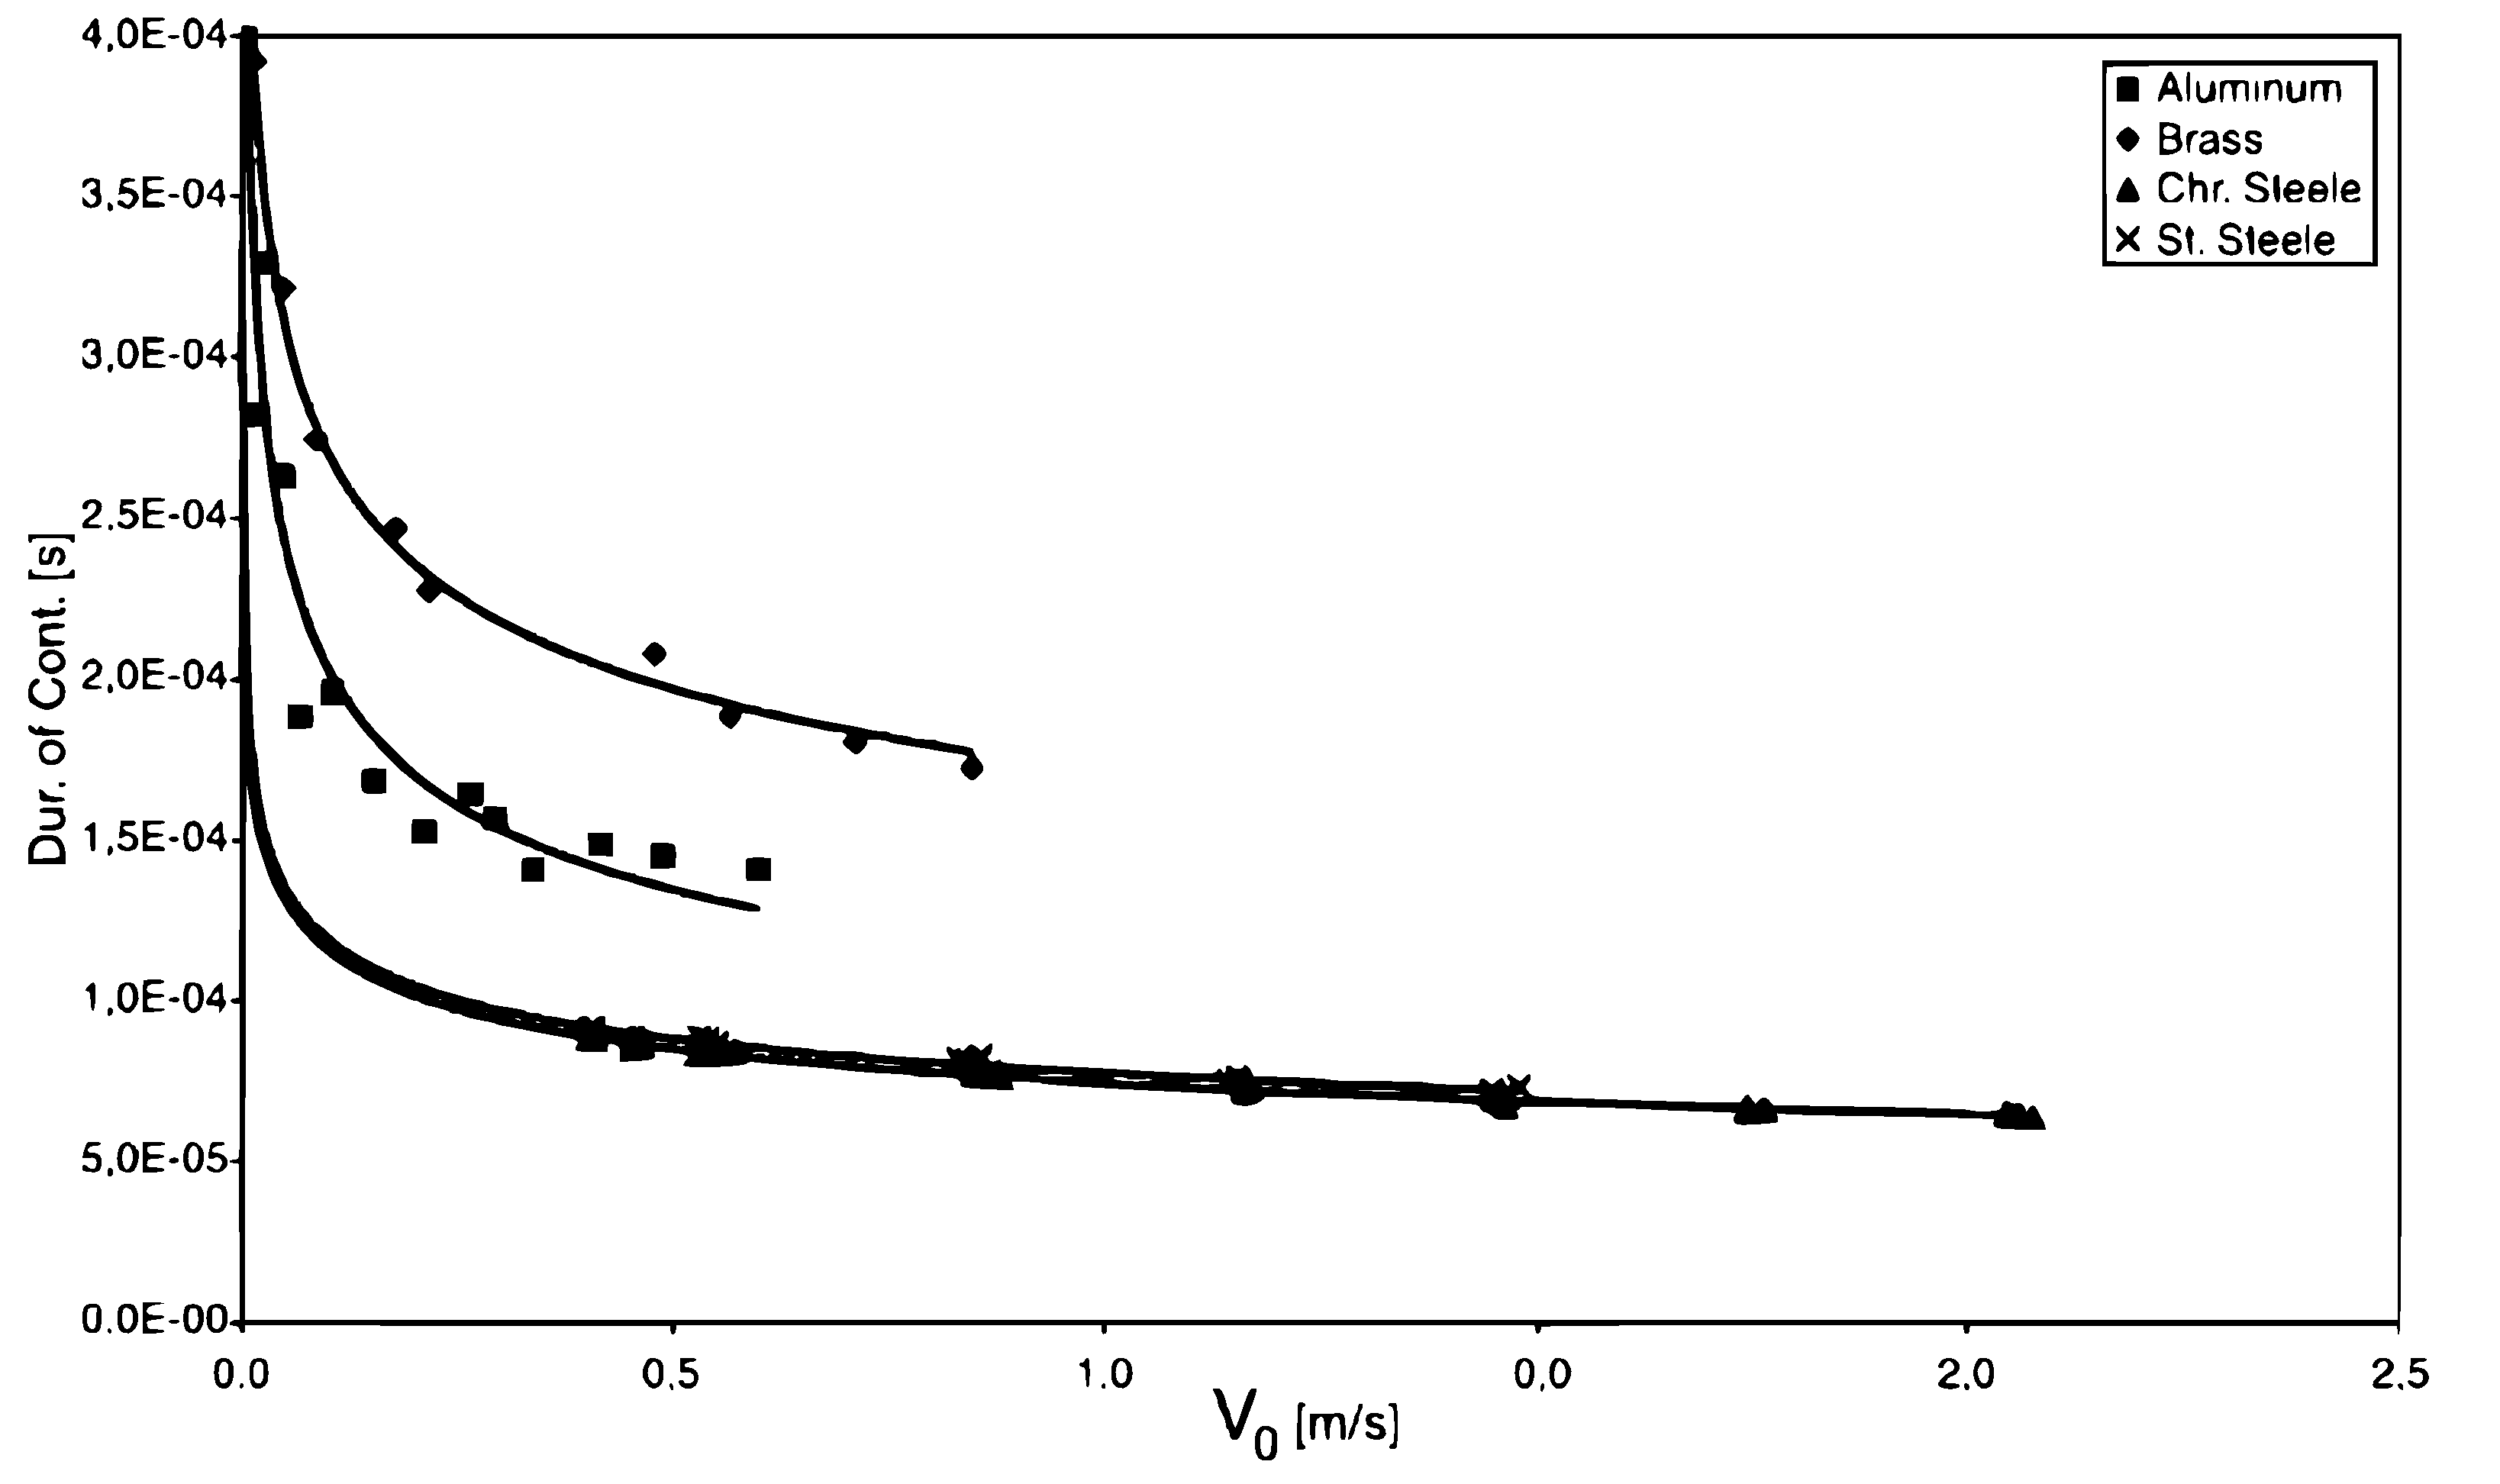
\includegraphics[width=0.80\linewidth]{Figures/3.Chapter/impact_time}
%	\caption{Duration of contact $t_c$ as a function of the impact normal velocity $V_0$ \citep{Kruggel-Emden-2007}.}
%	\label{fig:t_c_exp} 
%\end{figure}
%

Non-linear models allow to overcome the limitation imposed by a constant restitution coefficient and contact duration. \cite{Kuwabara-1987}, \cite{Brilliantov-1996} and \cite{Brilliantov-2001} proposed a fully non-linear model that reads

\begin{equation} \label{eq:non_linear_hertz_normal}
	\ve{F}_{n,ij}=\ve{F}_n^r+\ve{F}_n^d=k_{n,ij}\delta_{ij}^{3/2}\ve{e}_{ij}-\gamma_{n,ij}\delta_{ij}^{1/2}\dot{\delta}_{ij}\ve{e}_{ij},
\end{equation}
%
The stiffness, recovering the elastic Hertz model from Section \ref{sec:solid_model}, is given by a form of Equation \eqref{eq:hertz_III} 

%
\begin{equation} \label{eq:rigidity_hertz}
	k_{n,ij}=\frac{4}{3}E^*\sqrt{R^*}
\end{equation}
%
Considering exclusively the repulsive part of Equation \eqref{eq:non_linear_hertz_normal}, \cite{Shaefer-1996} notes that $t_{c,ij}$ is no longer independent from the normal velocity impact $v_{n,ij}$

%
\begin{equation} \label{eq:non_linear_tc}
	t_{c,ij}=3.21 \left( -\frac{M^*}{k_{n,ij}} \right)^{2/5}v_{n,ij}^{-1/5}
\end{equation}
%
implying that there is no longer an intrinsic time scale to collisions, as expected from experimental data.

\cite{Brilliantov-1996} and \cite{Brilliantov-2001} proposed that the viscous damper coefficient $\gamma_{n,ij}$ is a material property, obtainable from the bulk viscosities of the materials in collision and the local curvature at impact point. However, very little studies have been devoted to bulk viscosities and as a consequence $\gamma_{n,ij}$ is traditionally treated as a calibration parameter. \cite{Cummins-2011} writes an expression for $\gamma_{n,ij}$ depending exclusively on a normal restitution coefficient

%
\begin{equation} \label{eq:gamma_dem}
	\gamma_{n,ij}=-\frac{\log{e_{n,ij}}}{\sqrt{\pi^2+\log^2{e_{n,ij}}}}
\end{equation}
%
Expression \eqref{eq:gamma_dem} used in the context of a non-linear model, is ambiguous. In practice, a constant value for $e_{n,ij}$ will be used to compute $\gamma_{n,ij}$, that will lead to a non-constant, effective $e_{n,ij}$, depending on the impact velocity.

Figure \ref{fig:e_hertz} shows $e_{n,ij}$ as a function of $v_{n,ij}$, for the linear model and for the non-linear Hertz model (Expression \eqref{eq:non_linear_hertz_normal})

%
\begin{figure}[ht!]
	\centering
	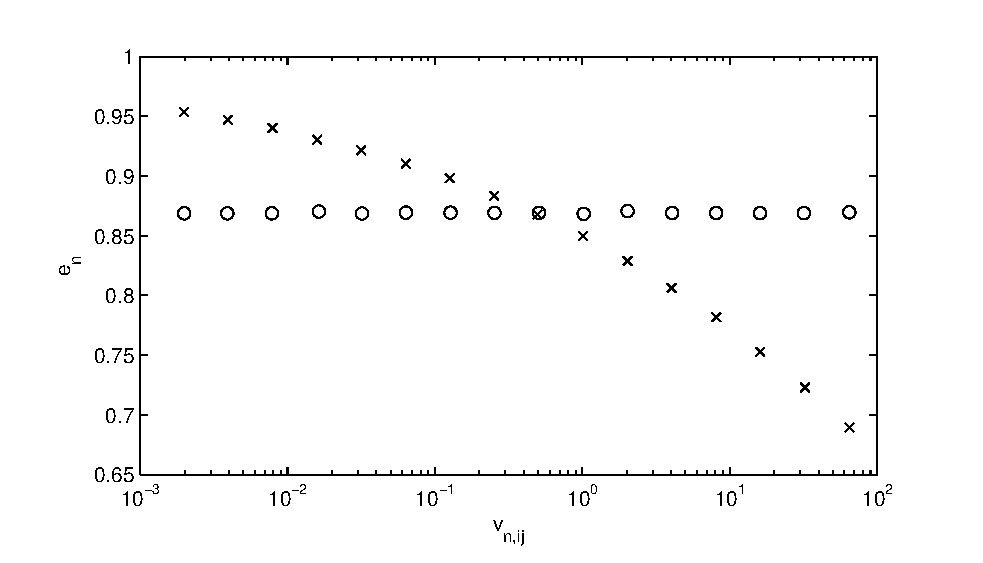
\includegraphics[width=0.80\linewidth]{Figures/3.Chapter/e_hertz}
	\caption{Normal restitution coefficient $e_{n,ij}$ as a function of the impact normal velocity $v_{n,ij}$. Linear force ($\circ$), Non-linear Hertz ($\times$)}
	\label{fig:e_hertz} 
\end{figure}
%
For the linear case $k_n=7.32\times10^6$ Nm$^{-1}$ and $\gamma_n=2.06$ kg s$^{-1}$, resulting in $e_n=0.87$. For the non-linear model, $\gamma_n=190$ m$^{-1/2}$s$^{-1}$, in order to produce comparable $e_n$ in the selected $v_{n,ij}$ range. As expected, the linear model produces a constant $e_n$. Force \eqref{eq:non_linear_hertz_normal} leads to an inversely proportional $e_{n,ij}$ with $v_{n,ij}$, i.e., $(1-e_{n,ij})\sim v_{n,ij}^{1/5}$, in agreement with experimental results (Figure \ref{fig:Restitution_coeff}).


Regarding tangential contacts, friction is modeled using the same model, as indicated in Figure \ref{fig:dem_scheme}. The mechanism can be reproduced by a linear dash-pot 

%
\begin{equation} \label{eq:elastic_fric}
	\ve{F}_{t,ij}=\ve{F}_t^r+\ve{F}_t^d=k_{t,ij}\delta^t_{ij}\ve{e}^t_{ij}-\gamma_{t,ij}\dot{\delta}^t_{ij}\ve{e}^t_{ij}
\end{equation}
%
where the stiffness and damping constants are derived to be

%
\begin{equation} \label{eq:fric_coeffs}
	k_{t,ij}=2/7k_{n,ij}; \;\;\;\;\; \gamma_{t,ij}=2/7\gamma_{n,ij},
\end{equation}
%
as to insure internal consistency of the time scales required for stability \citep{Hoomans-2000}. This mechanism models the static and dynamic friction mechanisms by a penalty method. The body does not statically stick at the point of contact, but is constrained by the spring-damper system. This force must be bounded above by the Coulomb friction law introduced by Equation \eqref{eq:coulomb_friction}. The Coulomb law is modified with a sigmoidal function in order to make it continuous around the origin regarding the tangential velocity \citep{Vetsch-2011}:

%
\begin{equation} \label{eq:fric_I}
	\ve{F}_{t,ij}=\min(\mu_{fIJ} \ve{F}_{n,ij} \tanh (8\dot{\delta}^t_{ij})\ve{e}^t_{ij};\;\; \ve{F}_{t,ij}),
\end{equation}
%
\noindent where $\mu_{fIJ}$ is the friction coefficient at the contact of $I$ and $J$ and is simply taken as the average of the two friction coefficients of the distinct materials.